\documentclass[hyperref={bookmarks=false},aspectratio=169]{beamer}
\usepackage[utf8]{inputenc}
\usepackage{hyperref}
\usepackage{natbib}

\usepackage[croatian]{babel}
% ---------------  Define theme and color scheme  -----------------
\usetheme[sidebarleft]{Caltech}  % 3 options: minimal, sidebarleft, sidebarright

%\setbeamertemplate{footline}[frame number]

% ------------  Information on the title page  --------------------
\title[Grafička sučelja za git]
{\bfseries{Grafička sučelja za git}}



\author[Sandro Šafar \and Stella Dumenić\and Robin Šćulac]
{}

\institute[Riteh]


\date[25.1.2019.]
{Računalne vještine, računarstvo, 1. godina}
%------------------------------------------------------------

%------------------------------------------------------------
%The next block of commands puts the table of contents at the 
%beginning of each section and highlights the current section:

\AtBeginSection[]
{
  \begin{frame}
    \frametitle{Tablica Sadržaja}
    \tableofcontents[currentsection]

  \end{frame}
}
%------------------------------------------------------------


\begin{document}
\frame{\titlepage}  % Creates title page

%---------   table of contents after title page  ------------
%\begin{frame}
%\frametitle{Table of Contents}
%\tableofcontents
%\end{frame}
%---------------------------------------------------------


\section{gitflow}

\begin{frame}

\frametitle{Gitflow}
Gitflow je model grananja gita u kojem postoje dvije grane:

\begin{itemize}
    \item master 
    \item develop

\end{itemize}

Master grana je spremna za objavljivanje projekta dok develop grana služi za poboljšavanje ili dodavanje elemenata.

\end{frame}



\section{vrste gitflow sučelja}


\begin{frame}
\frametitle{TortoiseGit}

\begin{block}{\tiny{Općenito}}
Open source sučelje namijenjeno za Windows
\end{block}
\begin{block}{Prednosti}

    \begin{itemize}
    \item jednostavan za koristiti 
    \item issue tracking system
    \item korisni alati
    \item dostupan u mnogo jezika
    \item stabilan
    \item sadrži spell check, auto completion
    \item besplatan za koristiti
    \end{itemize}
\end{block}
\end{frame}

\begin{frame}{TortoiseGit}
    
    \begin{columns}
\frametitle{TortoiseGit}
\column{0.75\textwidth}
\begin{figure}



\includegraphics[width=\columnwidth]{./figures/tortoisegit.png}
    \centering
    
\end{figure}
\column{0.25\textwidth}
    
\end{columns}
    

\end{frame}
%------------------------------------------------------

\begin{frame}
\frametitle{Aurees}

    
\begin{block}{\tiny{Općenito}}
Git sučelje namijenjeno za Windows i Mac korisnike. Uskoro dolazi verzija i za Linux.
\end{block}

\begin{block}{Prednosti}
    
    \begin{itemize}
        \item jednostavan za koristiti
        \item prikazuje commit-ove u "side by side" text editoru
        \item zanimljiv i jednostavan prikaz korisnika i izmjena
        \item besplatan za privatne korisnike
    \end{itemize}
\end{block}

\end{frame}

\begin{frame}{Aurees}
    
    \begin{columns}
\frametitle{Aurees}
\column{0.75\textwidth}
\begin{figure}


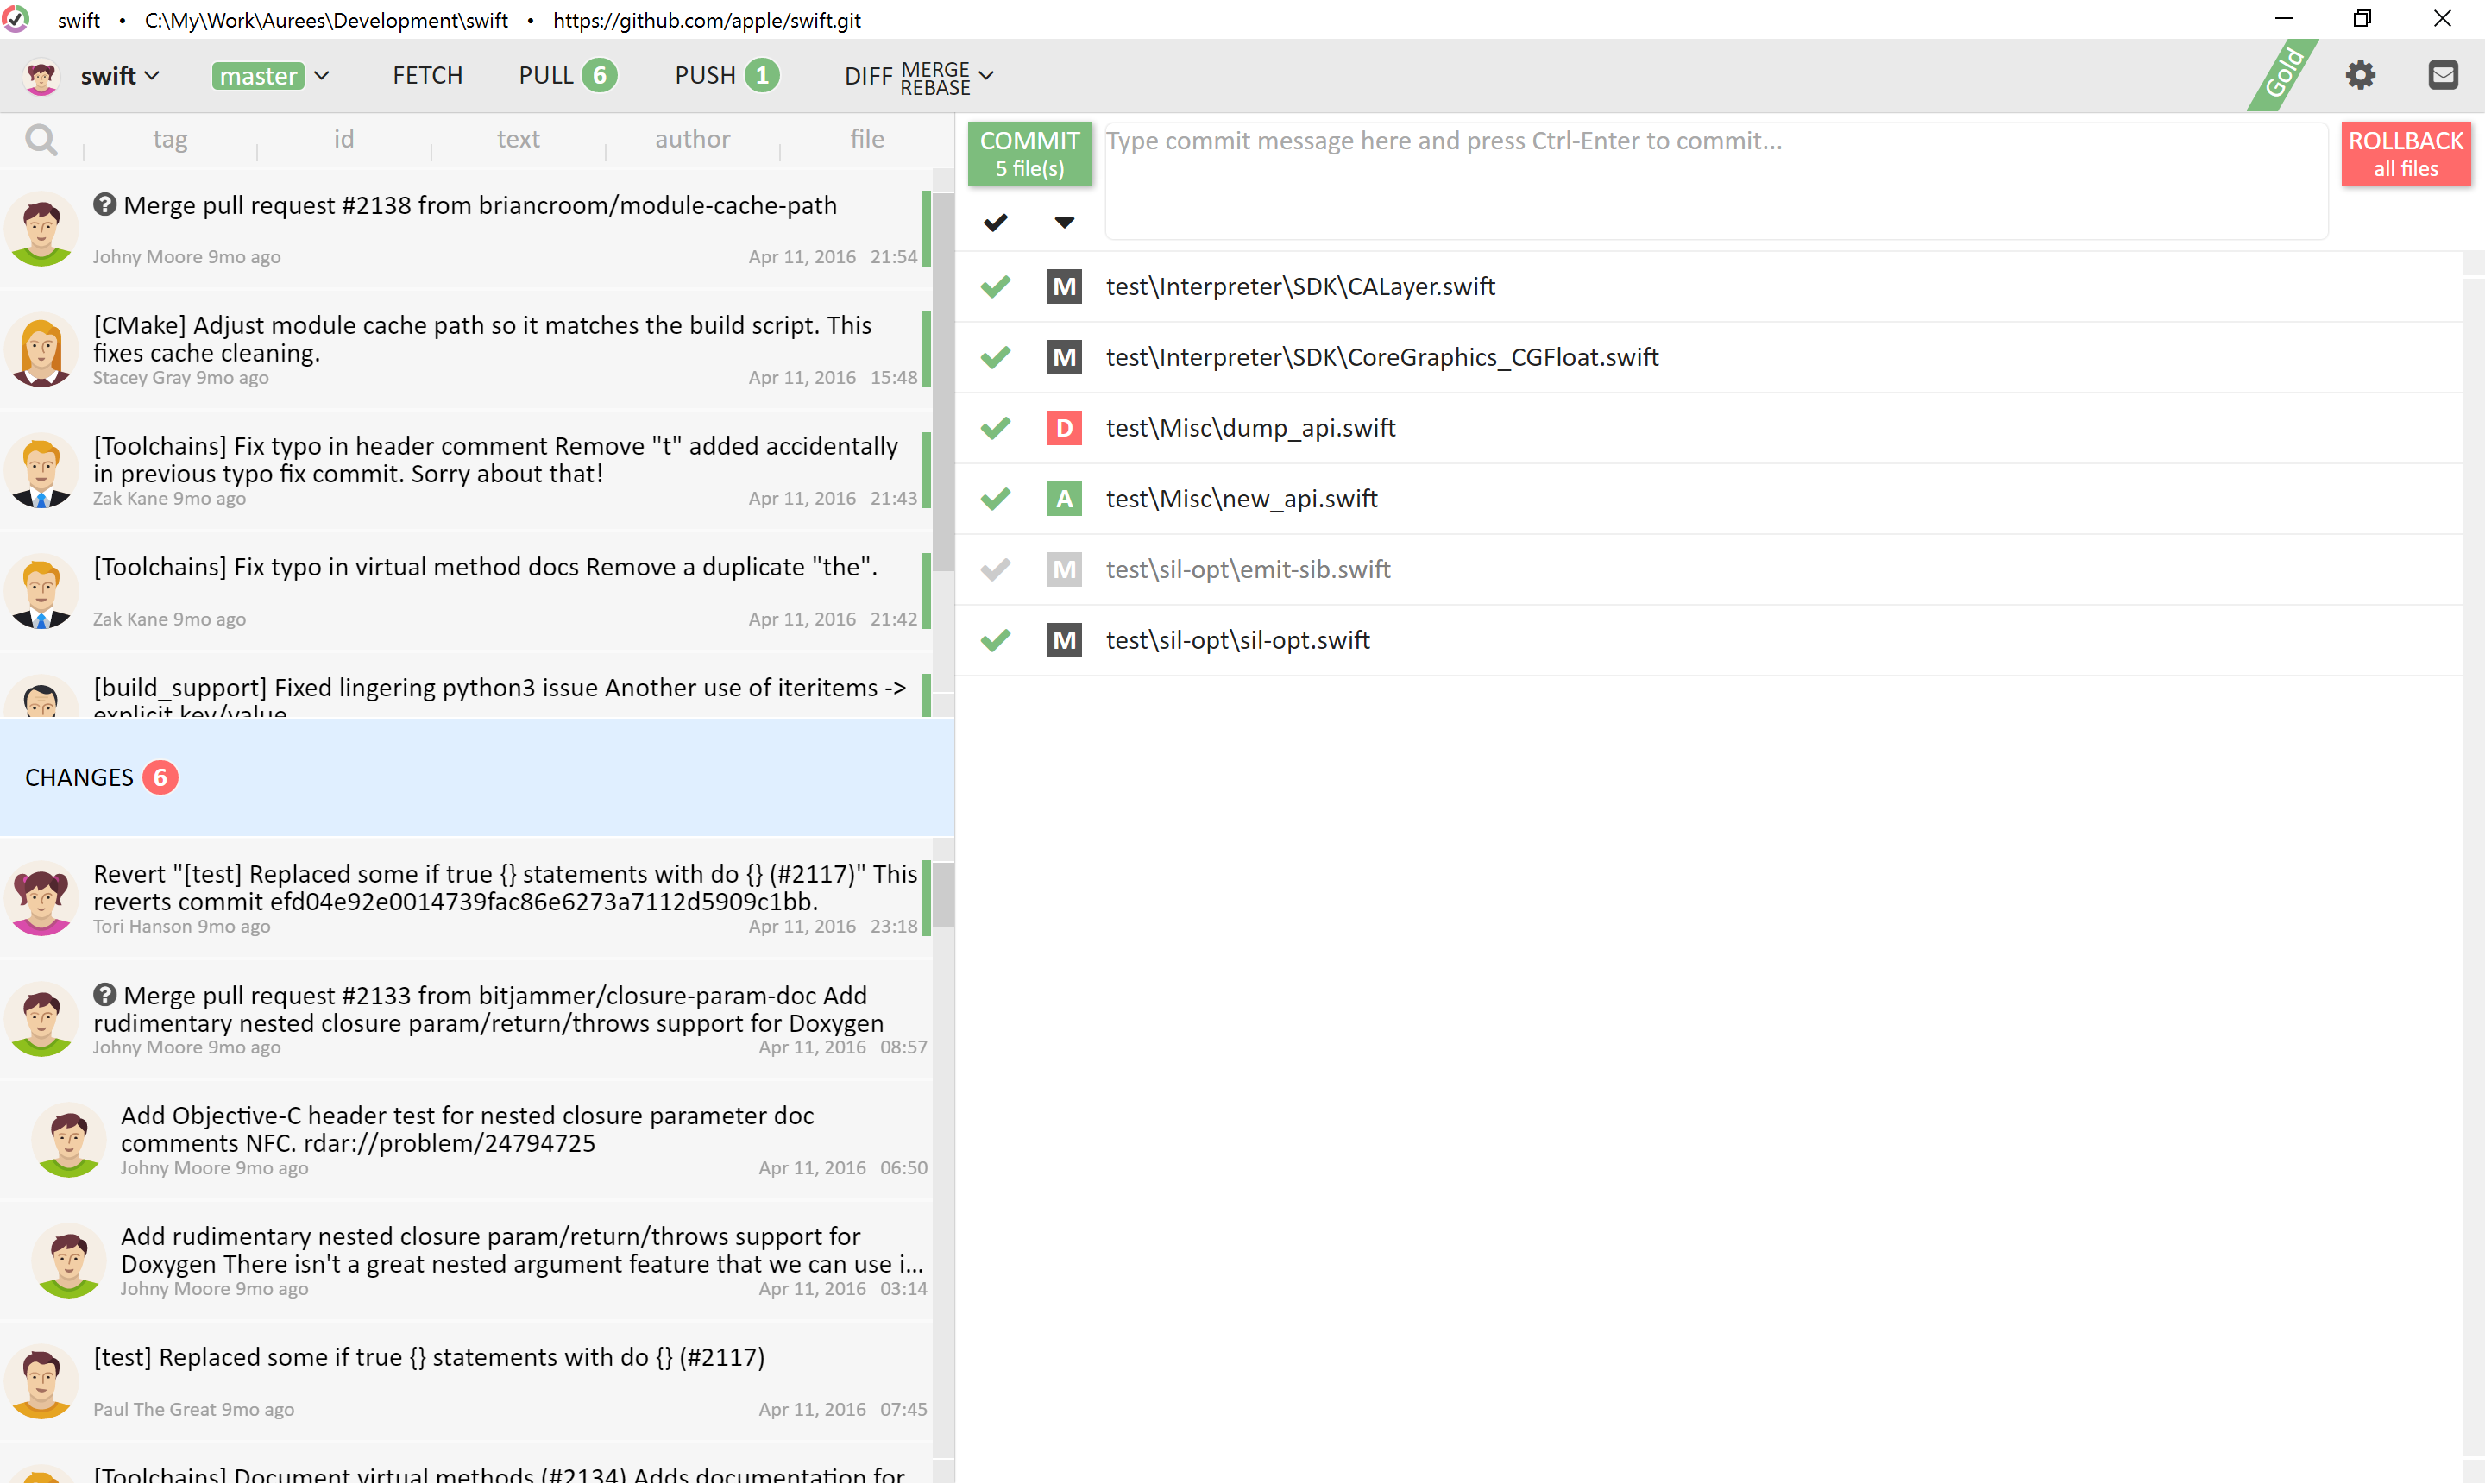
\includegraphics[width=\columnwidth]{./figures/aurees.png}
    \centering
    
\end{figure}
\column{0.25\textwidth}
    Prikaz Aurees sučelja
\end{columns}
    

\end{frame}


%------------------------------------------------------kraken
\begin{frame}
\begin{columns}
\frametitle{GitKraken}
\column{0.45\textwidth}
\begin{figure}


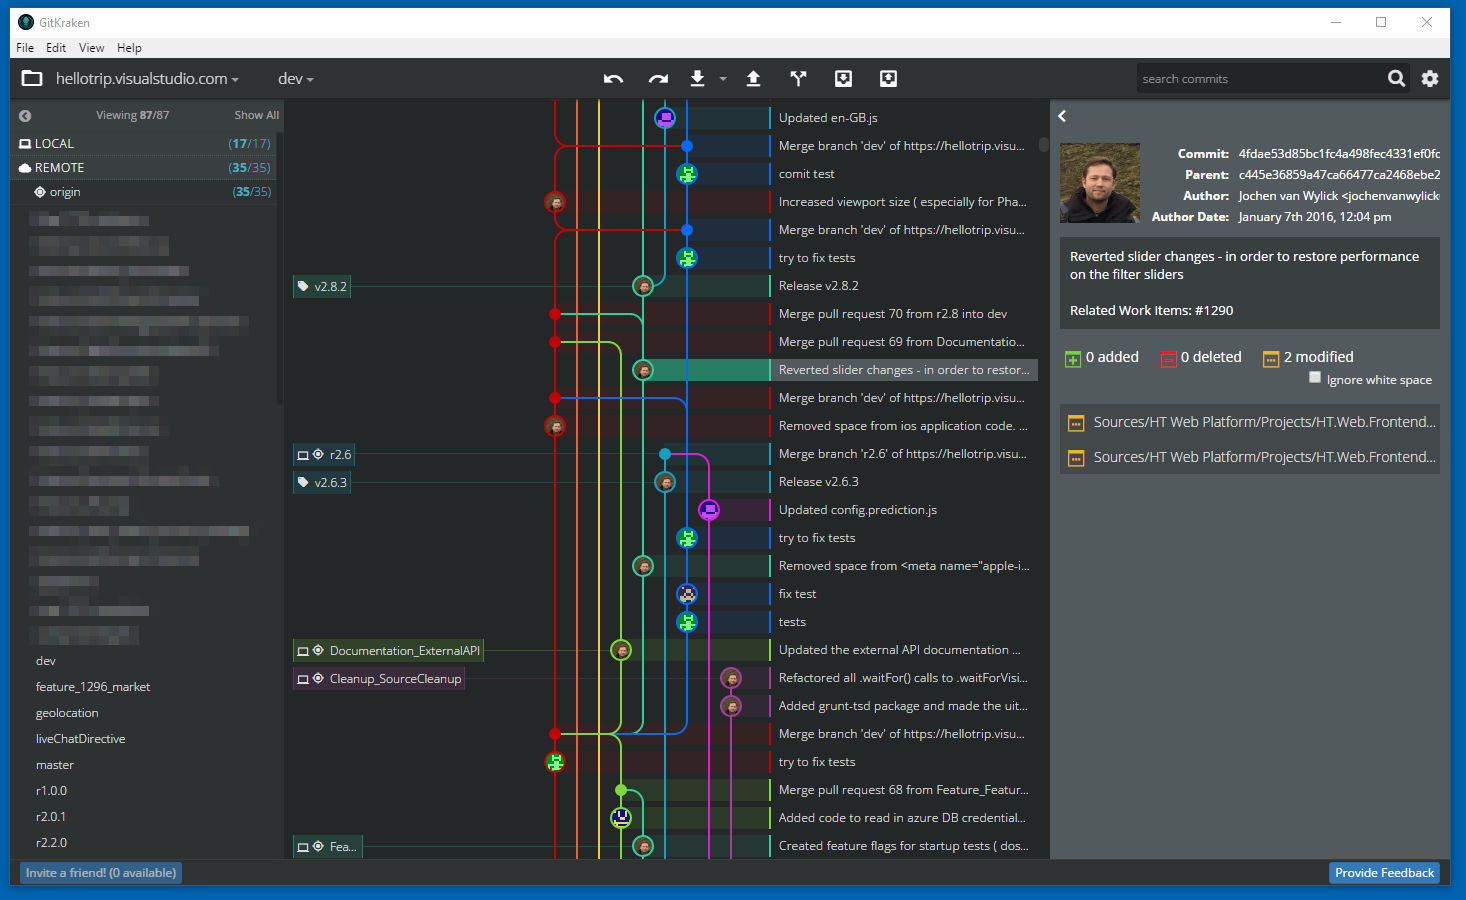
\includegraphics[width=\columnwidth]{./figures/git_kraken.png}
    \centering
    \caption{GUI od Git krakena  \emph{\\grafovi commit poruke i autori}}
\end{figure}
\column{0.55\textwidth}
    GitKraken je git sučelje dizajnirano da u prvi plan stavlja korisničku intuitivnost
\begin{itemize}
    \item jednostavan Drag & Drop sustav
    \item jednostavan prikaz brancheva i povijesti commitova
\end{itemize}
\end{columns}

\end{frame}




%---------------------------------------------------------git hub desktop
\begin{frame}
\begin{columns}
\frametitle{GitHub Desktop}
\column{0.45\textwidth}
\begin{figure}


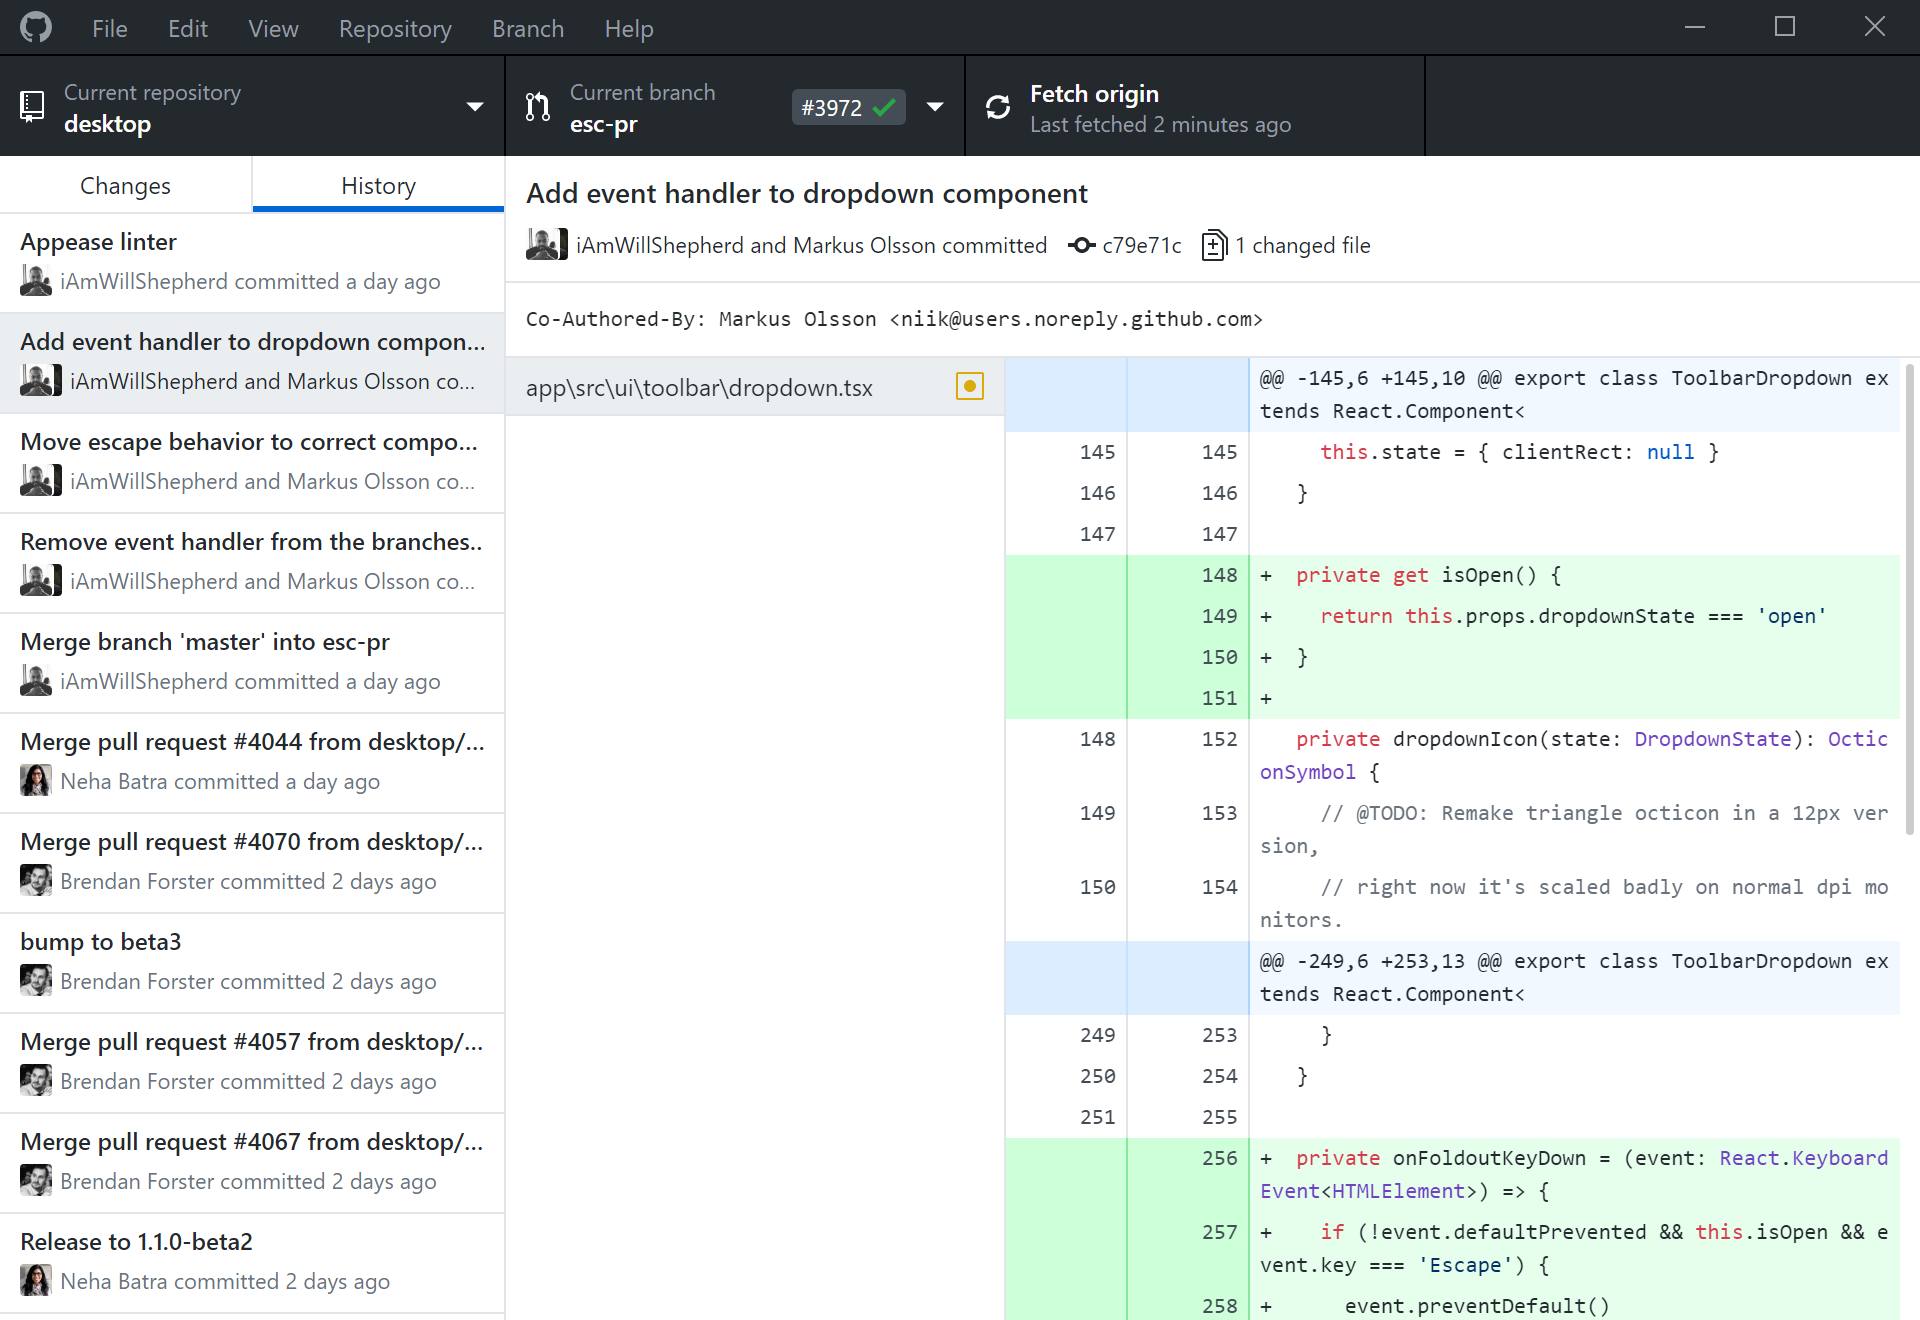
\includegraphics[width=\columnwidth]{./figures/github-desktop-screenshot-windows.png}
    \centering
    \caption{GUI od GitHubDesktopa  \emph{\\slika skinuta sa https://desktop.github.com/}}
\end{figure}
\column{0.55\textwidth}
\begin{itemize}
    \item ekstenzija GitHuba
    \item olakšava pretraživanje GitHubovih repozitorija
    \item datoteke su pakirane nevjerovatnom brzinom (u uspordebi s GitKrakenom)
    \end{itemize}
    nedostaci:
    \begin{itemize}
     \item kompleksniji od ostalih sučelja
     \item ograničenje za slanje podataka
\end{itemize}
 
\end{columns}

\end{frame}
%------------------------------------------------------sandro
\begin{frame}

\frametitle{SmartGit}

\begin{enumerate}

\item \underline{\textbf{Isto}} grafičko sučelje na Windowsu, macOSu i Linuxu
    
\item Globalna SmartGit licenca (može se koristiti  \underline{\textbf{bilo gdje}})\\
    
\item \textbf{Prilagođavanje potrebama.\\}
    
 Moguća konfiguracija na razne načine:\\
\fontsize{0.55cm}{0.4cm}\selectfont
\begin{itemize}
\item Preference merge-a i rebase-a
\item Raspored određenih elemenata
\item Vanjske alate
\item Vanjske ili ugrađene Compare ili Conflict Solver alate
\item Tipkovničke prečace
\item Toolbare
\item Boju sintakse
\item Svjetle i tamne teme
\end{itemize}

    

\end{enumerate}




\end{frame}

%------------------------------------------------------

\begin{frame}
\frametitle{SmartGit}
\begin{columns}

\column{0.55\textwidth}
\textbf{\underline{Nema potrebe za dodatnim alatima\\}}\\\

SmartGit uključuje:

\begin{itemize}
   \item Komandnu liniju (Windows, macOS)
   \item Grafičku Merge i Commit povijest
   \item Git-Flow
   \item SSH
   \item Compare datoteka
   \item Merge datoteka ("Conflict Solver" - trostruki merge)
\end{itemize}

\column{0.45\textwidth}

\begin{figure}
    \centering
    
\includegraphics[width=\columnwidth]{./figures/SmartGit-logo.jpg}
    \caption{SmartGit logo}
    \tiny{(Photo downloaded from: https://linuxhint.com\\/wp-content/uploads/2016/04/SmartGit-logo.jpg)}
    \label{fig:smartgit-logo}
\end{figure}

\end{columns}

\end{frame}

%------------------------------------------------------
\begin{frame}
\frametitle{SmartGit}
\textbf{\underline{Interakcija s popularnim platformama}}\\\

Sadrži posebne integracije za \textbf{GitHub}, \textbf{BitBucket} i \textbf{BitBucket Server} (prijašnji \textbf{Atlassian Stash)} za stvaranje i rješavanje Pull Requestova i pregledavanje komentara\\\

Može se koristiti i sa vlastitim Git repozitorijima ili drugim hosting poslužiteljima (npr. GitLab)\\\

SmartGit možete preuzeti \textbf{\href{https://www.syntevo.com/smartgit/}{ovdje.}}


\end{frame}

%------------------------------------------------------
\begin{frame}
\frametitle{GitEye}

\begin{block}{Glavne značajke}
\begin{enumerate}
    \item \large{\textbf{User-friendly\\}}
    \small{Jednostavna instalacija te pregledno sučelje}\\\
    \item \large{\textbf{Potpuna povijest\\}}
    \small{Mogućnost uvida u povijest svake linije koda}\\\
    \item \large{\textbf{Integracija\\}}
    \small{Mogućnost povezivanja s vanjskim poslužiteljima i alatima (npr. GitHub)}\\\
    \item \large{\textbf{Windows, Linux i macOS\\}}

\end{enumerate}
\end{block}

\end{frame}
%------------------------------------------------------
\begin{frame}
\frametitle{Dostupnost grafičkih sučelja}
\begin{center}
\begin{tabular}{ |c||c | c | c| } 
 \hline
 \multirow{Sučelje}&\multicolumn{3}{c|}{OS}\\ 
 \cline{2-4}
 & Windows & Linux & macOS \\
 \hline
 TortoiseGit & + & - & - \\
 \hline
 Aurees & + & - & + \\ 
 \hline
 SmartGit & + & + & + \\ 
 \hline
 GitEye & + & + & + \\ 
 \hline
  GitHub Desktop & + & - & + \\ 
 \hline
  GitKraken & + & + & + \\ 
 \hline
\end{tabular}
\end{center}

\end{frame}
%------------------------------------------------------Literatura

\begin{frame}{Literatura}
\printbibliography
\begin{thebibliography}{9}
\bibitem{GUI Clients} Biblioteka svih sučelja:
\url{https://git-scm.com/downloads/guis/}
\bibitem{TortoiseGit}TortoiseGit:
\url{https://tortoisegit.org/}

\bibitem{Aurees} Aurees:
\url{https://aurees.com//}

\bibitem{GitKraken} GItKraken:
\url{ https://www.gitkraken.com/}

\bibitem{GitHubDesktop}Git Hub Desktop:
\url{https://desktop.github.com/}

\bibitem{SmartGit} Smart Git:
\url{https://www.syntevo.com/smartgit/}

\bibitem{gitEye} GitEye:
\url{https://www.collab.net/products/giteye}

\end{thebibliography}
\end{frame}


\end{document}
